\documentclass[a4paper,12pt]{article}

\usepackage[utf8]{inputenc}
\usepackage[spanish]{babel}
\usepackage{amsmath, amssymb}
\usepackage{graphicx}
\usepackage{float}
\usepackage{booktabs}
\usepackage{xcolor}
\usepackage{listings}
\usepackage{caption}
\usepackage{fancyhdr}
\usepackage{hyperref}
\usepackage{tikz}

\hypersetup{
    colorlinks=true,
    linkcolor=blue,
    urlcolor=blue,
    pdftitle={Práctica 4 - ESP32},
}
% ---------- PREÁMBULO: arreglar comillas en listings (Thonny style) ----------
\usepackage[utf8]{inputenc}   % si no está ya
\usepackage[T1]{fontenc}      % mejor soporte de tipografías para PDFs
\usepackage{textcomp}         % símbolos de texto adicionales
\usepackage{upquote}          % comillas ' y " tipo ASCII en verbatim/listings

% Si usas babel con español, desactiva el shorthand de la comilla doble
\usepackage[spanish]{babel}
\shorthandoff{"}  % <<< evita que " sea un caracter activo (causa comillas invisibles)

% Colores inspirados en Thonny
\usepackage{xcolor}
\definecolor{thonnyKeyword}{rgb}{0.0,0.2,0.8}
\definecolor{thonnyComment}{rgb}{0.0,0.5,0.0}
\definecolor{thonnyString}{rgb}{0.7,0.12,0.12}
\definecolor{thonnyBackground}{rgb}{1.0,1.0,1.0}
\definecolor{thonnyBuiltin}{rgb}{0.5,0.0,0.5}
\definecolor{thonnyNumber}{rgb}{0.35,0.35,0.35}

% Declaración de lenguaje MicroPython (basado en Python)
\usepackage{listings}
\lstdefinelanguage{MicroPython}{
    morekeywords={
        False, True, None, and, as, assert, async, await, break, class, continue,
        def, del, elif, else, except, finally, for, from, global, if, import,
        in, is, lambda, nonlocal, not, or, pass, raise, return, try, while, with, yield
    },
    morekeywords=[2]{print,open,range,len,abs,int,float,str,dict,list,set,tuple},
    morekeywords=[3]{machine,network,time,urequests,utime,gc,Pin,ADC,PWM,UART,RTC,ESP32},
    sensitive=true,
    morecomment=[l]{\#},
    morestring=[b]",
    morestring=[b]',
}

% Configuración de listings con estilo Thonny (y upquote activo)
\lstset{
    language=MicroPython,
    backgroundcolor=\color{thonnyBackground},
    keywordstyle=\color{thonnyKeyword}\bfseries,
    keywordstyle=[2]\color{thonnyBuiltin},
    keywordstyle=[3]\color{thonnyKeyword!60!black},
    commentstyle=\color{thonnyComment}\itshape,
    stringstyle=\color{thonnyString},
    numberstyle=\tiny\color{thonnyNumber},
    basicstyle=\ttfamily\small,
    numbers=left,
    numbersep=6pt,
    frame=single,
    framerule=0.4pt,
    breaklines=true,
    breakatwhitespace=true,
    showstringspaces=false,
    tabsize=2,
    captionpos=b,
    columns=flexible,
    upquote=true     % importante para mostrar comillas rectas correctamente
}
% -------------------------------------------------------------------------


\title{Práctica N°4: Uso de Adafruit en ESP32 con comunicación Wi-Fi}
\date{}

\begin{document}
\maketitle
\tableofcontents
\newpage

\section{Objetivos}

\subsection{Objetivo General}
Configurar y programar una placa ESP32 para establecer comunicación con la plataforma Adafruit IO mediante el protocolo MQTT, permitiendo el envío y recepción de datos entre un sensor local (potenciómetro) y un tablero virtual en la nube.

\subsection{Objetivos Específicos}
\begin{itemize}
    \item Registrar y configurar una cuenta en Adafruit IO, creando los \textit{feeds} necesarios para la comunicación con el ESP32.
    \item Implementar la conexión Wi-Fi del ESP32 y establecer un cliente MQTT utilizando las librerías de MicroPython.
    \item Programar el envío periódico de datos analógicos (lectura de potenciómetro) hacia la nube y la recepción de comandos para el control de un LED remoto.
    \item Analizar el flujo de comunicación entre el dispositivo y el servidor Adafruit IO, comprendiendo los procesos de publicación, suscripción y callback.
\end{itemize}

\section{Configuración de Adafruit IO desde la Web}

Antes de poder ejecutar el código en el ESP32, es necesario realizar la configuración de la cuenta y los elementos correspondientes en la plataforma \textbf{Adafruit IO}. Esta etapa permitirá establecer la comunicación entre el dispositivo físico y la nube mediante el protocolo MQTT.

\subsection{Creación de cuenta y acceso al panel principal}

Para iniciar, se debe acceder al sitio oficial de Adafruit IO (\url{https://io.Adafruit.com}) y crear una cuenta gratuita. Una vez registrado, el usuario puede ingresar al panel principal, donde se gestionan los \textit{feeds}, \textit{dashboards} y \textit{keys} de acceso.

\begin{figure}[H]
    \centering
    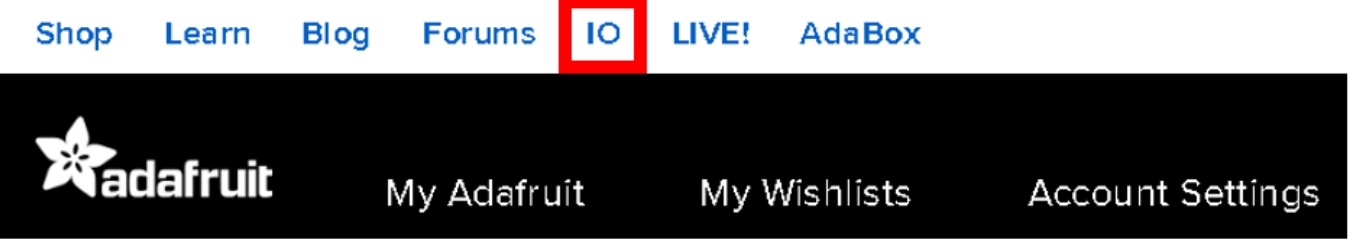
\includegraphics[width=0.8\textwidth]{Adafruit/Ada_IO.jpeg}
    \caption{Pantalla inicial de Adafruit IO y registro de usuario.}
\end{figure}

\subsection{Obtención de la clave de API (Adafruit IO Key)}

Desde el menú lateral, se debe acceder a la opción \textbf{“My Key”}, donde se muestran las credenciales personales necesarias para la conexión MQTT.  
Esta clave se utilizará dentro del código en la variable \texttt{AdafRUIT\_IO\_KEY}, permitiendo autenticar la sesión del ESP32 con el servidor.

\begin{figure}[H]
    \centering
    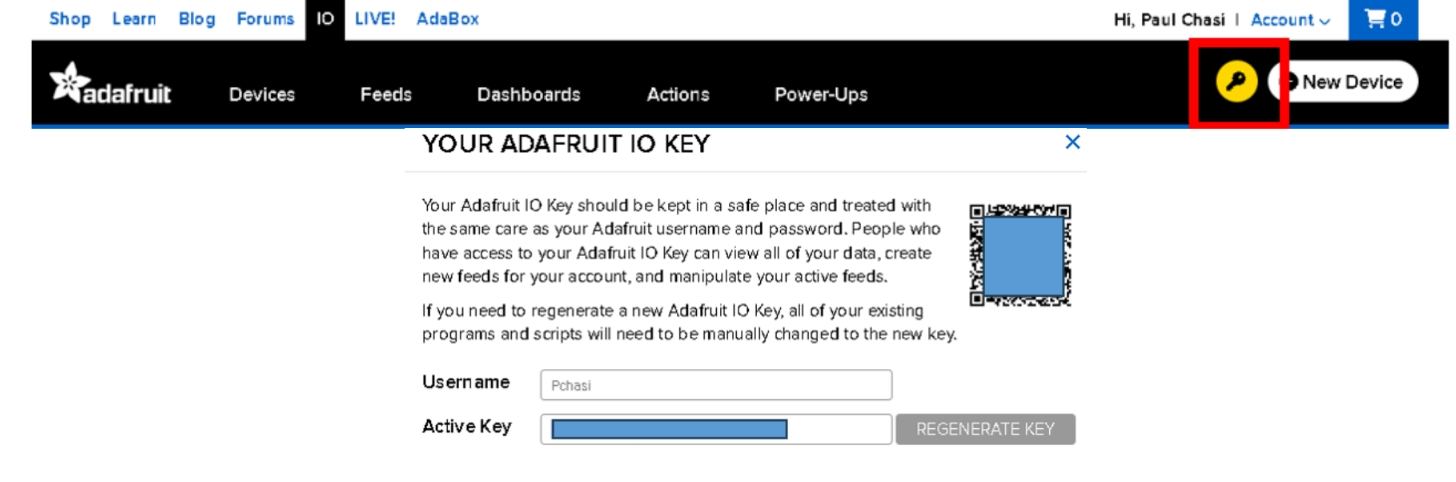
\includegraphics[width=0.8\textwidth]{Adafruit/Key.jpeg}
    \caption{Creación de un nuevo feed en Adafruit IO.}
\end{figure}

\subsection{Creación de los Feeds}

Los \textit{feeds} son los canales de comunicación entre la nube y el dispositivo.  
Para este proyecto se requieren dos:
\begin{itemize}
    \item \textbf{esp32.pulsante}: para recibir valores (0 o 1) y controlar el encendido del LED.
    \item \textbf{esp32.potenciometro}: para enviar el valor leído del potenciómetro desde el ESP32 hacia la nube.
\end{itemize}

Estos se crean desde el menú \textbf{Feeds > Actions > Create a New Feed}, asignando los nombres exactos que luego se referencian en el código.

\begin{figure}[H]
    \centering
    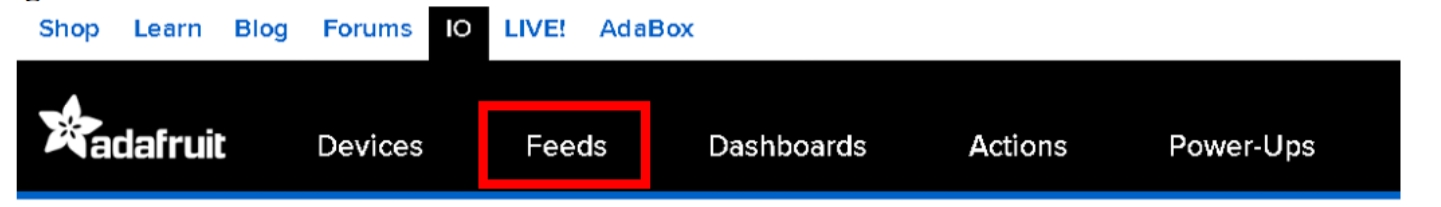
\includegraphics[width=0.8\textwidth]{Adafruit/Ada_feeds.jpeg}
    \caption{Ubicación de la clave de acceso (Adafruit IO Key) en la configuración de la cuenta.}
\end{figure}

\begin{figure}[H]
    \centering
    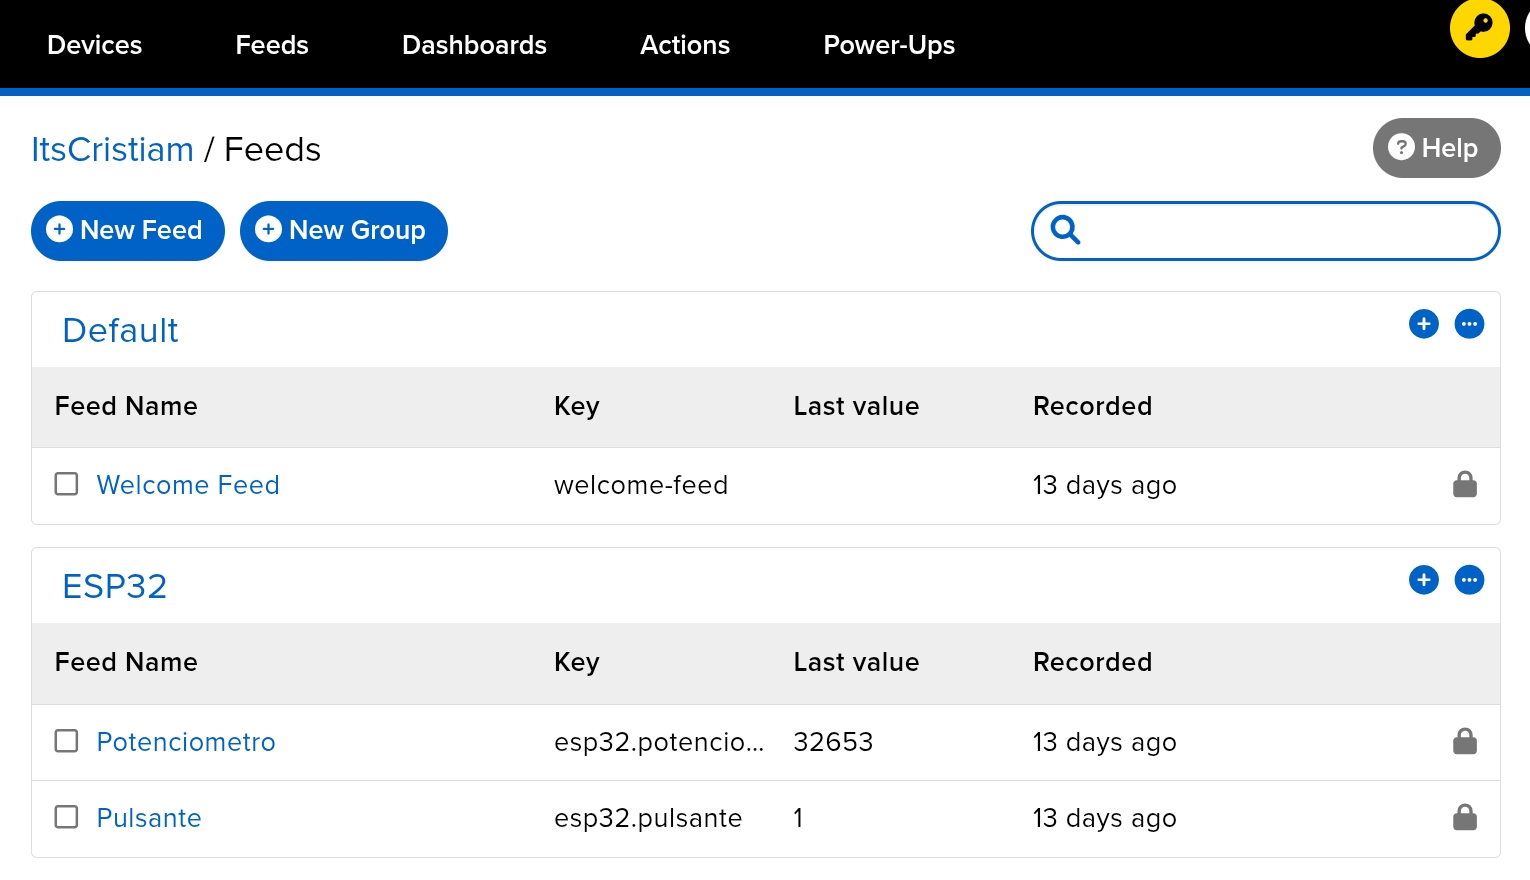
\includegraphics[width=0.8\textwidth]{Adafruit/Feeds.jpeg}
    \caption{Ubicación de la clave de acceso (Adafruit IO Key) en la configuración de la cuenta.}
\end{figure}

\subsection{Diseño del Dashboard}

Una vez creados los feeds, se recomienda construir un \textit{dashboard} para visualizar y controlar los datos.  
Desde \textbf{Dashboards > New Dashboard} se crea una interfaz donde se pueden agregar bloques interactivos:
\begin{itemize}
    \item Un \textbf{slider o gauge} vinculado al feed \texttt{esp32.potenciometro} para observar el valor analógico enviado por el potenciómetro.
    \item Un \textbf{toggle button} asociado al feed \texttt{esp32.pulsante} para enviar el valor 0/1 al ESP32 y controlar el LED.
\end{itemize}

\begin{figure}[H]
    \centering
    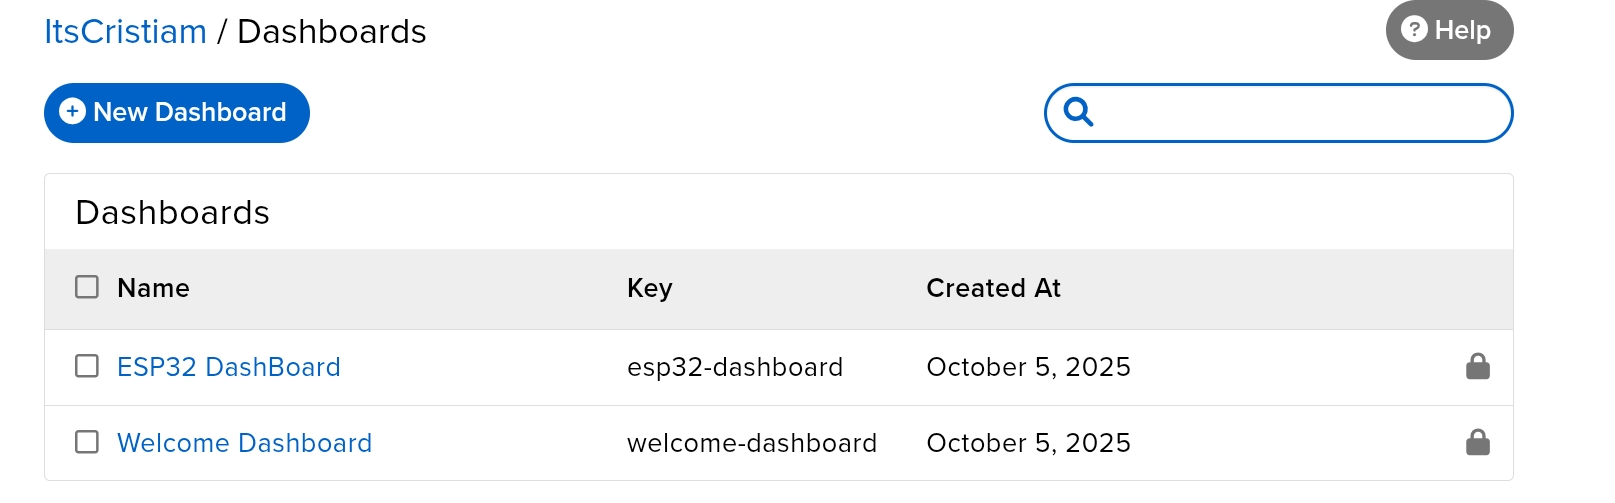
\includegraphics[width=0.8\textwidth]{Adafruit/Dash_menu.jpeg}
    \caption{Configuración de bloques en el Dashboard y asociación con los feeds.}
\end{figure}

\begin{figure}[H]
    \centering
    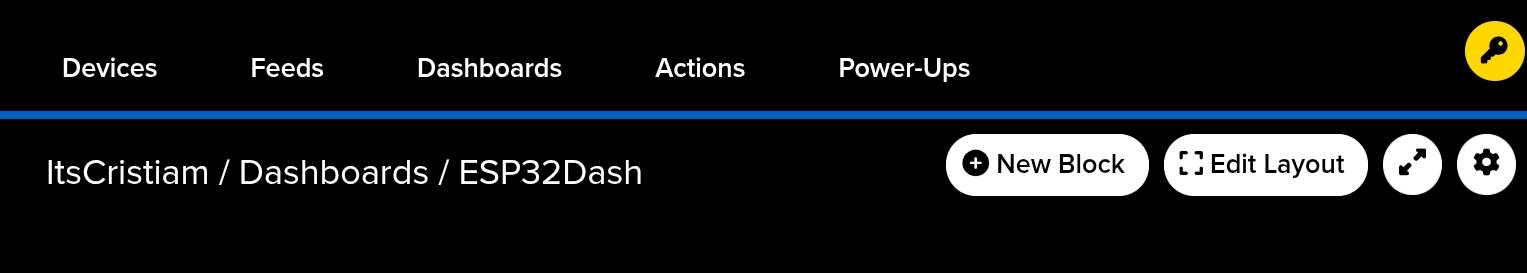
\includegraphics[width=0.8\textwidth]{Adafruit/Dash_0.jpeg}
    \caption{Configuración de bloques en el Dashboard y asociación con los feeds.}
\end{figure}

\begin{figure}[H]
    \centering
    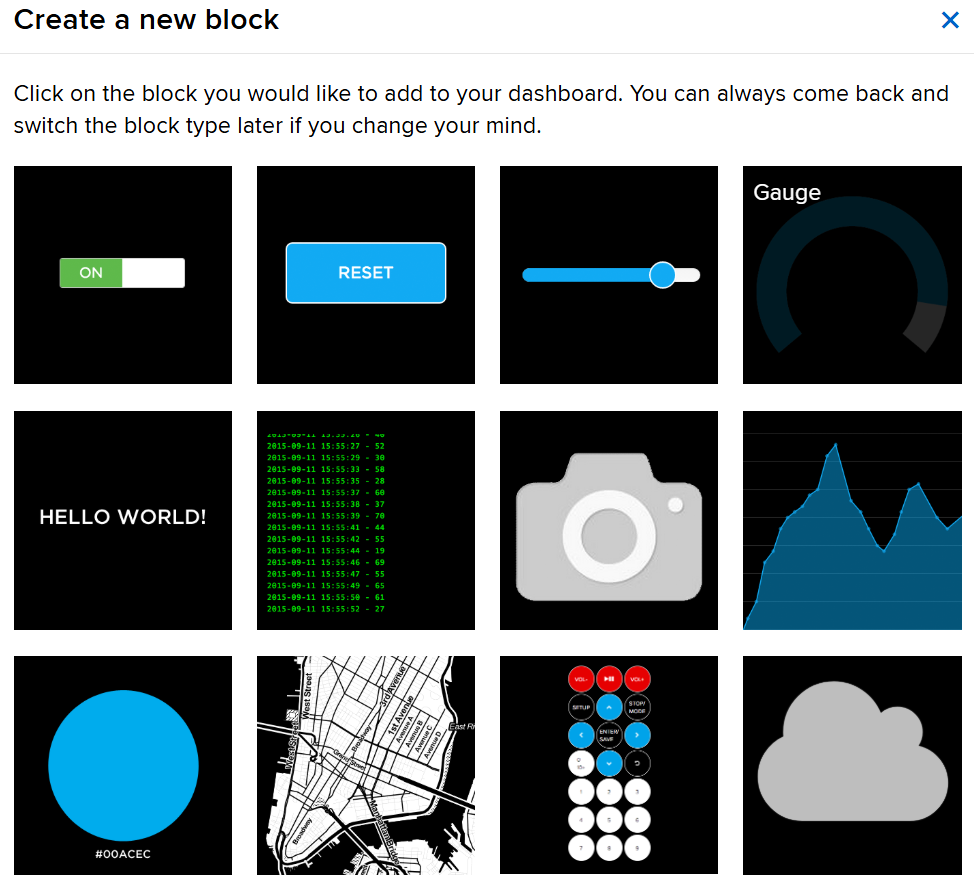
\includegraphics[width=0.8\textwidth]{Adafruit/menu_creat.png}
    \caption{Configuración de bloques en el Dashboard y asociación con los feeds.}
\end{figure}

\begin{figure}[H]
    \centering
    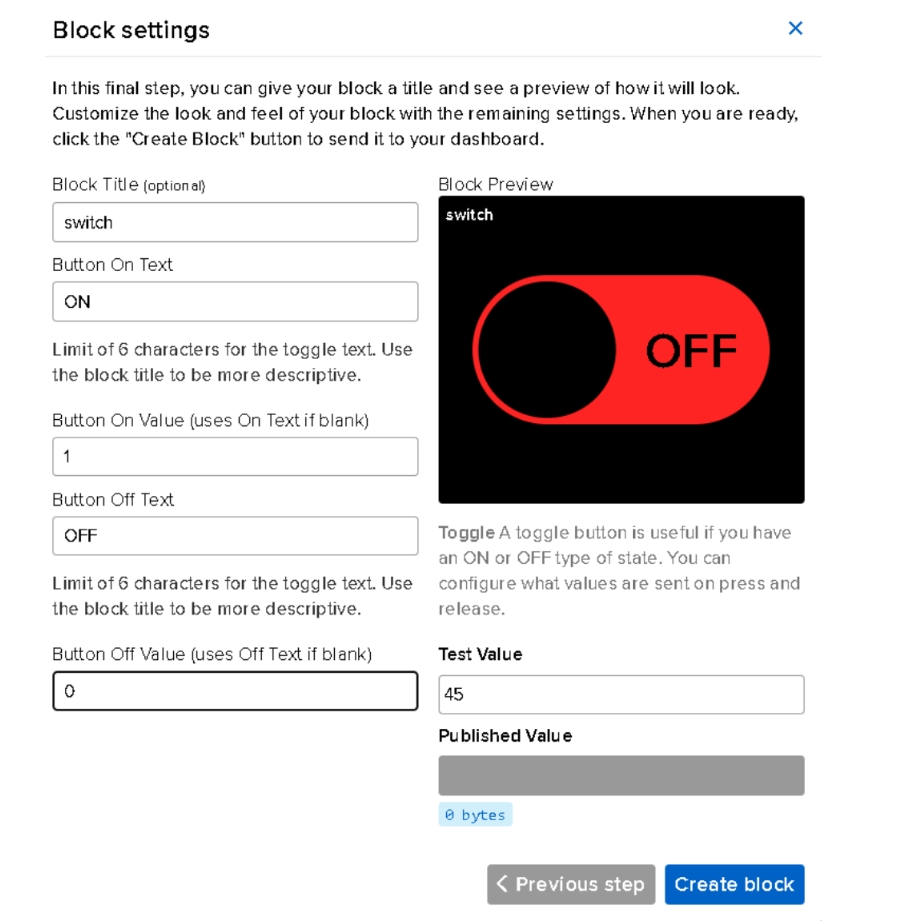
\includegraphics[width=0.8\textwidth]{Adafruit/LED_sett.jpeg}
    \caption{Configuración de bloques en el Dashboard y asociación con los feeds.}
\end{figure}

\begin{figure}[H]
    \centering
    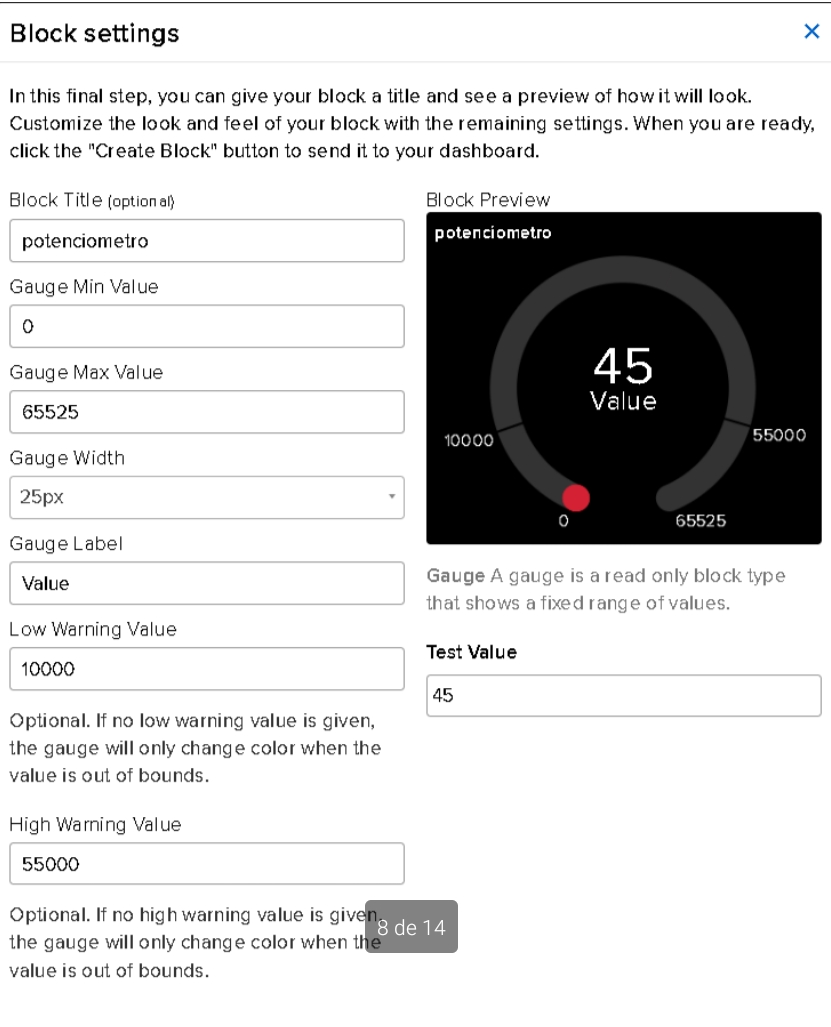
\includegraphics[width=0.6\textwidth]{Adafruit/Pot_sett.jpeg}
    \caption{Configuración de bloques en el Dashboard y asociación con los feeds.}
\end{figure}

\begin{figure}[H]
    \centering
    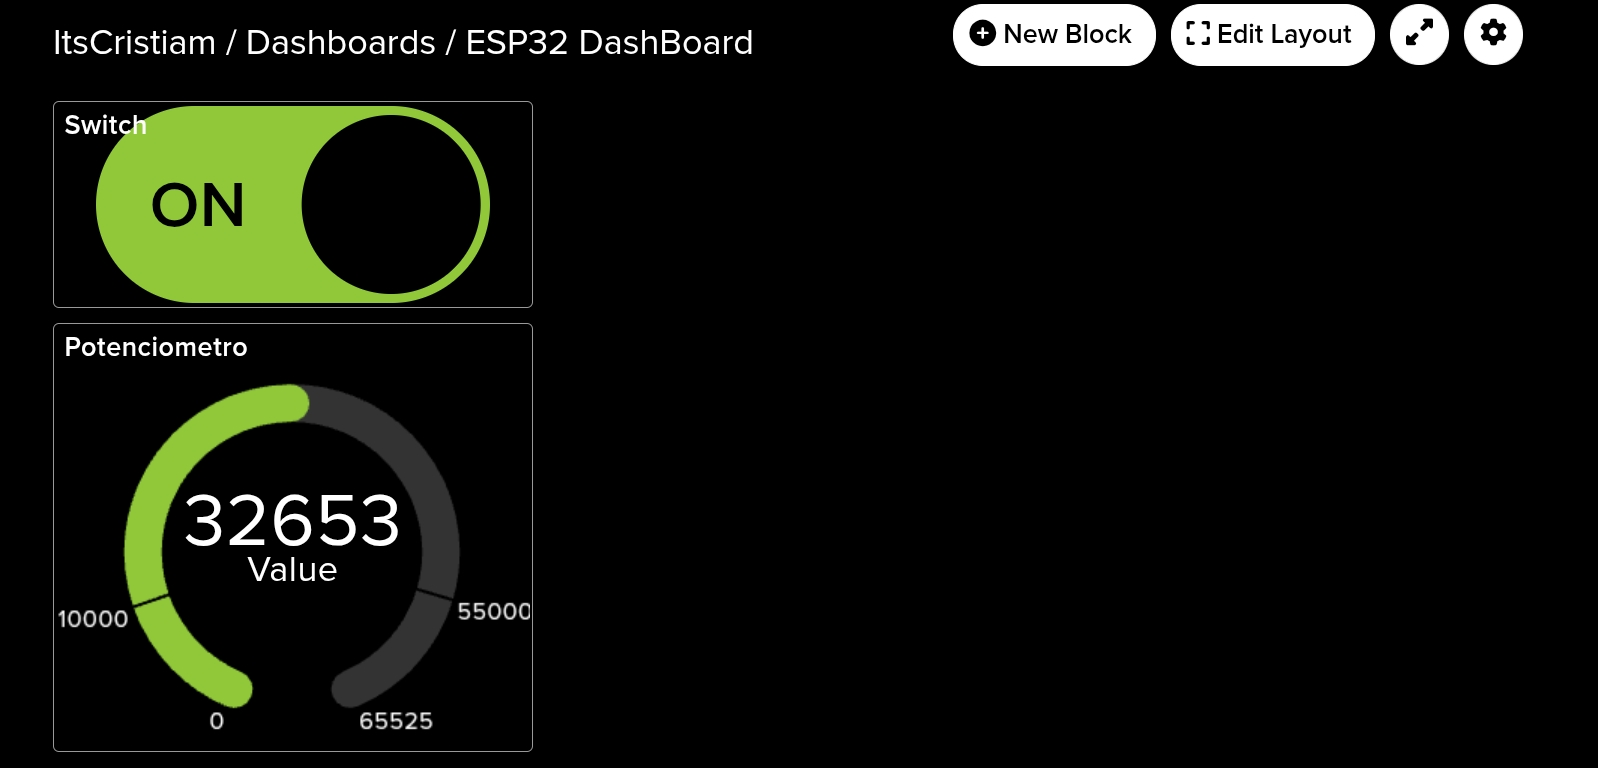
\includegraphics[width=0.8\textwidth]{Adafruit/Dash_final.jpeg}
    \caption{Configuración de bloques en el Dashboard y asociación con los feeds.}
\end{figure}


Con estos pasos completados, la plataforma Adafruit IO queda preparada para interactuar con el programa implementado en el ESP32, permitiendo analizar posteriormente el funcionamiento del código, la lógica de conexión y el intercambio de datos mediante MQTT.

\section{Explicación del Código}

En esta sección se presenta el desarrollo del programa implementado en el microcontrolador \textbf{ESP32} para la comunicación con la plataforma \textbf{Adafruit IO}.  
El código fue escrito en \textbf{MicroPython} y utiliza el protocolo \textbf{MQTT} para enviar y recibir datos entre el dispositivo y la nube.

\subsection{Código completo}

\begin{lstlisting}[language=Python, caption={Código completo para conexión ESP32 -- Adafruit IO en MicroPython.}]
# main.py - ESP32 MicroPython (Adafruit IO publish + subscribe)
# Requiere: umqtt.simple o umqtt.robust (subir a la placa o instalar via upip)

import network
import time
import sys
from machine import Pin, ADC

# --------- CONFIGURA AQUI ----------
SSID = "TU_RED_WIFI"
PASSWORD = "TU_CONTRASENA"

AdafRUIT_USERNAME = "TU_USUARIO_AdafRUIT"
AdafRUIT_IO_KEY = "TU_CLAVE_IO"
AdafRUIT_IO_SERVER = "io.adafruit.com"
AdafRUIT_IO_PORT = 1883

FEED_LED = "esp32.pulsante"
FEED_POT = "esp32.potenciometro"
# -----------------------------------

# Pines ESP32: LED y lectura analogica
LED_PIN = 2
POT_PIN = 34

led = Pin(LED_PIN, Pin.OUT)
adc = ADC(Pin(POT_PIN))
adc.atten(ADC.ATTN_11DB)
adc.width(ADC.WIDTH_12BIT)

# Intentar importar MQTT robusto
try:
    from umqtt.robust import MQTTClient
except Exception:
    from umqtt.simple import MQTTClient

# Funcion para leer ADC (0 a 65535)
def read_adc_u16(adc_obj):
    try:
        return int(adc_obj.read_u16())
    except Exception:
        v = adc_obj.read()
        return int((v * 65535) // 4095)

# Generar topics MQTT
def topic_for(feedname):
    return "{}/feeds/{}".format(AdafRUIT_USERNAME, feedname)

# Callback de mensajes recibidos
def mqtt_callback(topic, msg):
    t = topic.decode()
    m = msg.decode()
    print("MSG IN ->", t, ":", m)
    if FEED_LED in t:
        if m.strip() == '0':
            led.value(0)
        else:
            led.value(1)

# Conexion WiFi
def wifi_connect():
    wlan = network.WLAN(network.STA_IF)
    wlan.active(True)
    if not wlan.isconnected():
        print("Conectando a WiFi...")
        wlan.connect(SSID, PASSWORD)
        while not wlan.isconnected():
            time.sleep(0.5)
    print("Conectado a:", wlan.ifconfig()[0])

# Conexion MQTT y suscripcion
def mqtt_connect_and_subscribe():
    client_id = "esp32-" + str(int(time.time()))
    client = MQTTClient(client_id, AdafRUIT_IO_SERVER,
                        AdafRUIT_IO_PORT, AdafRUIT_USERNAME,
                        AdafRUIT_IO_KEY)
    client.set_callback(mqtt_callback)
    print("Conectando a Adafruit IO MQTT...")
    client.connect()
    client.subscribe(topic_for(FEED_LED))
    print("Suscrito a feed:", FEED_LED)
    return client

# Bucle principal
def main():
    wifi_connect()
    client = mqtt_connect_and_subscribe()
    pot_topic = topic_for(FEED_POT)
    last_publish = 0
    publish_interval = 2

    while True:
        client.check_msg()
        now = time.time()
        if now - last_publish >= publish_interval:
            v = read_adc_u16(adc)
            client.publish(pot_topic, str(v))
            print("Publicado:", v)
            last_publish = now
        time.sleep(0.1)

if __name__ == "__main__":
    main()
\end{lstlisting}

\newpage

\subsection{Importación de librerías y configuración inicial}

\begin{lstlisting}[language=Python]
import network
import time
import sys
from machine import Pin, ADC
\end{lstlisting}

Estas librerías proporcionan las funciones básicas para el control del hardware y la comunicación:
\begin{itemize}
    \item \texttt{network}: maneja la conexión Wi-Fi del ESP32.
    \item \texttt{machine}: permite acceder a los pines digitales y al ADC para leer el potenciómetro.
    \item \texttt{time} y \texttt{sys}: se emplean para temporización y manejo de errores.
\end{itemize}

\subsection{Declaración de credenciales y configuración del sistema}

\begin{lstlisting}[language=Python]
SSID = "TU_RED_WIFI"
PASSWORD = "TU_CONTRASENA"
AdafRUIT_USERNAME = "TU_USUARIO_AdafRUIT"
AdafRUIT_IO_KEY = "TU_CLAVE_IO"
\end{lstlisting}

El usuario debe reemplazar estas variables por los datos de su propia red Wi-Fi y cuenta de Adafruit IO.  
Esto permite que el dispositivo se autentique correctamente al momento de publicar o suscribirse a los \textit{feeds} definidos.

\subsection{Configuración de pines y del ADC}

\begin{lstlisting}[language=Python]
LED_PIN = 2
POT_PIN = 34
led = Pin(LED_PIN, Pin.OUT)
adc = ADC(Pin(POT_PIN))
adc.atten(ADC.ATTN_11DB)
adc.width(ADC.WIDTH_12BIT)
\end{lstlisting}

Aquí se establecen los pines físicos del ESP32:
\begin{itemize}
    \item El pin \texttt{GPIO2} controla un LED, que encenderá o apagará según la señal recibida.
    \item El pin \texttt{GPIO34} lee un valor analógico desde un potenciómetro.  
\end{itemize}
La configuración del ADC define una resolución de 12 bits (0–4095) y una atenuación de 11\,dB, lo que permite leer un rango aproximado de 0 a 3.6\,V.

\subsection{Conexión Wi-Fi}

\begin{lstlisting}[language=Python]
def wifi_connect():
    wlan = network.WLAN(network.STA_IF)
    wlan.active(True)
    if not wlan.isconnected():
        print("Conectando a WiFi...")
        wlan.connect(SSID, PASSWORD)
        while not wlan.isconnected():
            time.sleep(0.5)
    print("Conectado a:", wlan.ifconfig()[0])
\end{lstlisting}

Esta función activa la interfaz Wi-Fi del ESP32 y espera hasta que se establezca la conexión con el punto de acceso indicado.  
El método \texttt{ifconfig()} devuelve la dirección IP asignada, confirmando la conexión exitosa.

\subsection{Configuración del cliente MQTT}

\begin{lstlisting}[language=Python]
def mqtt_connect_and_subscribe():
    client_id = "esp32-" + str(int(time.time()))
    client = MQTTClient(client_id, AdafRUIT_IO_SERVER,
                        AdafRUIT_IO_PORT, AdafRUIT_USERNAME,
                        AdafRUIT_IO_KEY)
    client.set_callback(mqtt_callback)
    client.connect()
    client.subscribe(topic_for(FEED_LED))
    return client
\end{lstlisting}

Aquí se crea el cliente MQTT con los datos de usuario, servidor y puerto.  
La función \texttt{set\_callback()} asocia la rutina que procesará los mensajes recibidos.  
El ESP32 se suscribe al feed del LED para poder reaccionar a los comandos enviados desde Adafruit IO.

\newpage

\subsection{Recepción de mensajes (Callback)}

\begin{lstlisting}[language=Python]
def mqtt_callback(topic, msg):
    t = topic.decode()
    m = msg.decode()
    if FEED_LED in t:
        if m.strip() == '0':
            led.value(0)
        else:
            led.value(1)
\end{lstlisting}

El \textit{callback} interpreta los mensajes que llegan desde la nube.  
Cuando el usuario cambia el estado del botón en el dashboard, el ESP32 recibe un valor “0” o “1”, y enciende o apaga el LED según corresponda.

\subsection{Lectura del potenciómetro y publicación de datos}

\begin{lstlisting}[language=Python]
v = read_adc_u16(adc)
client.publish(pot_topic, str(v))
\end{lstlisting}

Cada cierto intervalo, el ESP32 lee el valor analógico del potenciómetro, lo convierte a una escala de 16 bits y lo publica en el feed correspondiente.  
Este valor puede visualizarse en tiempo real desde el panel de Adafruit IO mediante un bloque tipo \textit{gauge} o \textit{slider}.

\subsection{Bucle principal y verificación}

\begin{lstlisting}[language=Python]
while True:
    client.check_msg()
    now = time.time()
    if now - last_publish >= publish_interval:
        v = read_adc_u16(adc)
        client.publish(pot_topic, str(v))
        last_publish = now
    time.sleep(0.1)
\end{lstlisting}

El bucle principal mantiene activa la comunicación MQTT, verificando constantemente si hay nuevos mensajes y publicando datos del sensor de forma periódica.  
Este enfoque garantiza un flujo de información bidireccional entre el dispositivo físico y el entorno web.

\bigskip
Con esta estructura el estudiante puede modificar fácilmente los nombres de los feeds, los intervalos de publicación o incluso incorporar nuevos sensores, ampliando las posibilidades del proyecto IoT con Adafruit IO y ESP32.


\section{Resultados y Pruebas de Funcionamiento}

Una vez completada la configuración de la plataforma Adafruit IO y la carga del programa en el microcontrolador ESP32, se procede a verificar la comunicación bidireccional entre el hardware y la nube.  
El objetivo de esta fase es comprobar que los valores del potenciómetro se envíen correctamente al servidor y que el control remoto del LED responda a los comandos generados desde el \textit{dashboard}.

\subsection{Publicación de datos en Adafruit IO}

Durante la ejecución, el ESP32 realiza lecturas periódicas del potenciómetro y las publica en el feed configurado.  
En el panel web de Adafruit IO, este flujo de datos puede visualizarse en tiempo real mediante un bloque tipo \textit{gauge} o gráfico lineal, donde las variaciones del potenciómetro se reflejan en la interfaz.

\begin{figure}[H]
    \centering
    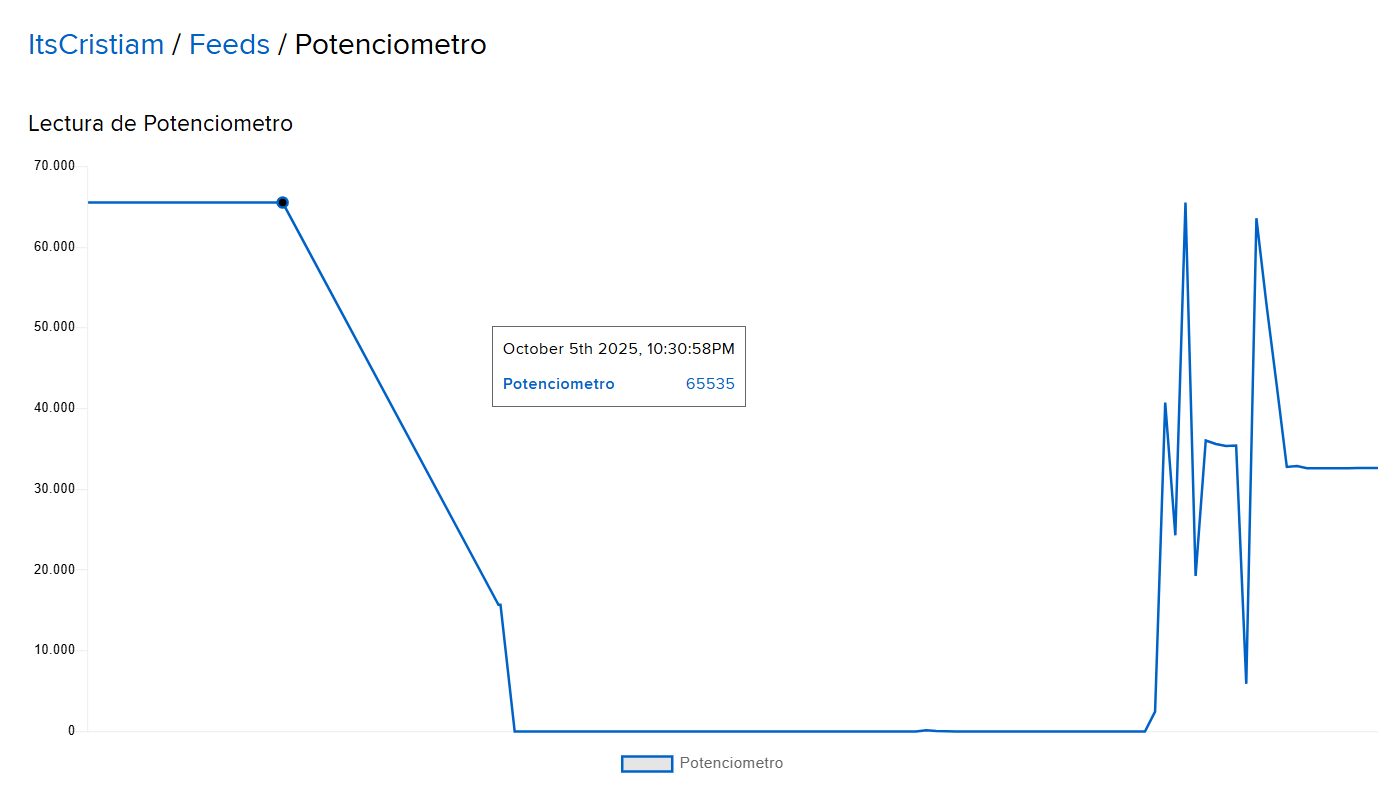
\includegraphics[width=0.85\textwidth]{Resultados/pot_result.png}
    \caption{Lectura del potenciómetro publicada en tiempo real en el feed \texttt{esp32.potenciometro}.}
\end{figure}

Cada envío incluye un valor numérico entre 0 y 65535 (equivalente al rango de lectura ADC de 16 bits), el cual se actualiza con una frecuencia determinada por la variable \texttt{publish\_interval} del código.

\subsection{Control remoto del LED desde el Dashboard}

El bloque de control del LED, configurado como un botón de tipo \textit{toggle}, permite enviar comandos “0” y “1” al feed \texttt{esp32.pulsante}.  
Cuando el usuario cambia el estado del botón en el dashboard, el mensaje MQTT se transmite a la placa, que ejecuta el \textit{callback} para encender o apagar el LED localmente.

\begin{figure}[H]
    \centering
    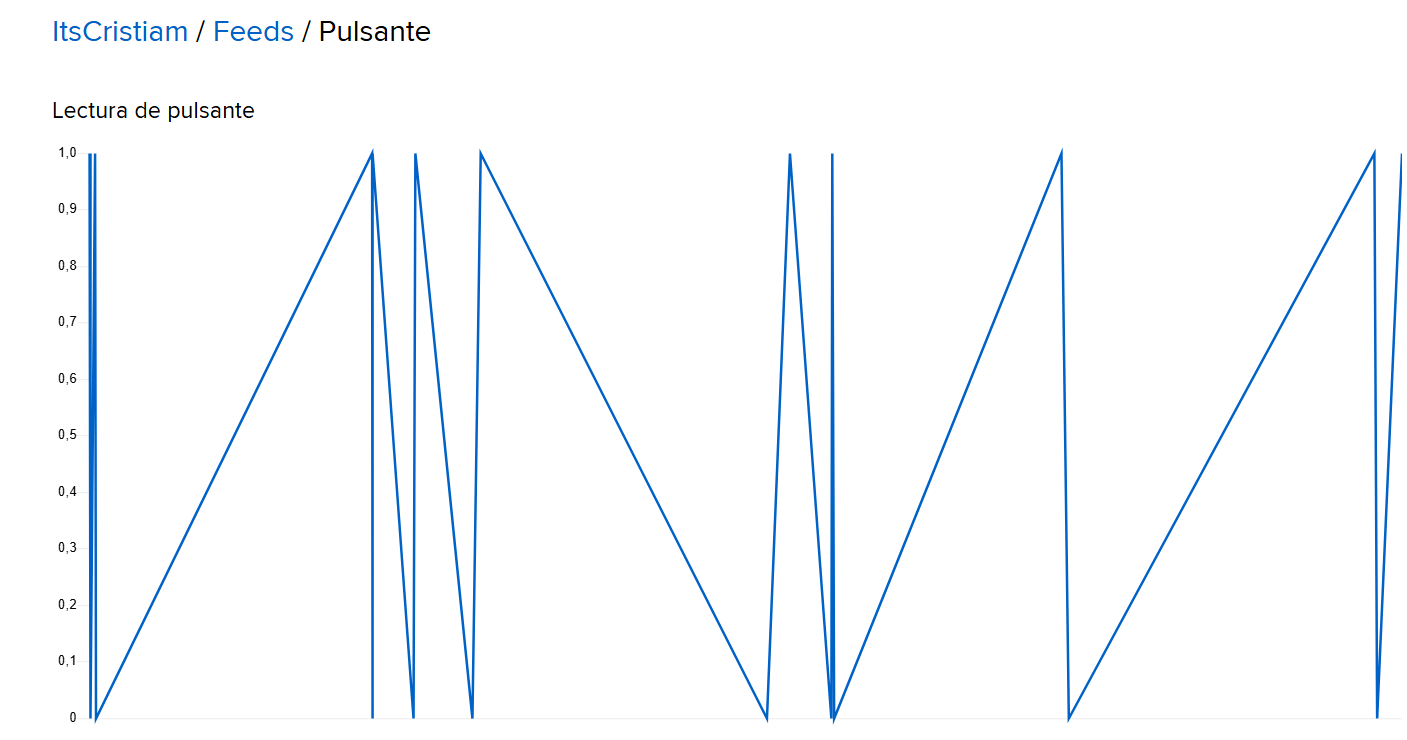
\includegraphics[width=0.85\textwidth]{Resultados/pulsante.png}
    \caption{Historial del feed de Adafruit IO con el control del LED remoto.}
\end{figure}

Este proceso confirma el funcionamiento correcto del canal de suscripción y demuestra la respuesta inmediata del sistema IoT.

\begin{figure}[H]
    \centering
    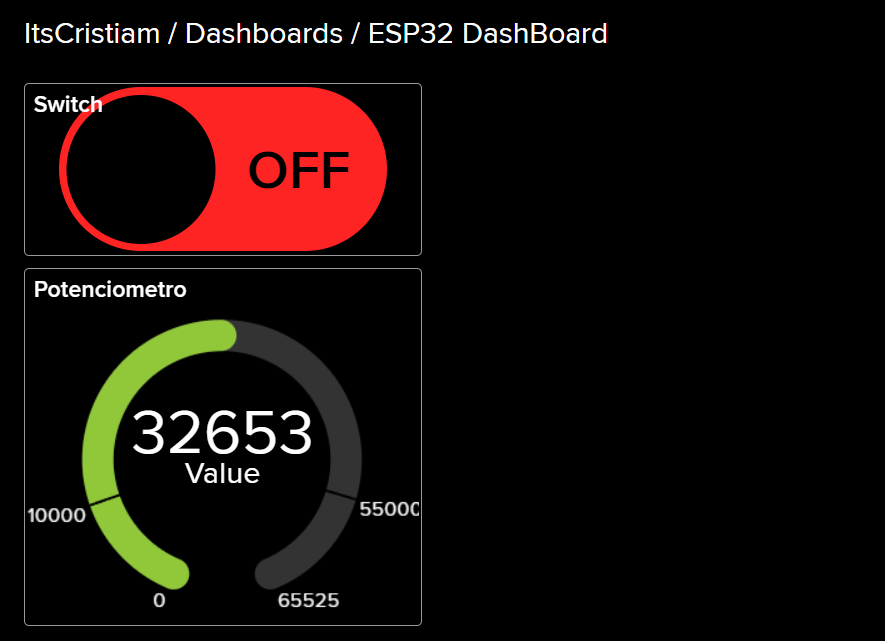
\includegraphics[width=0.65\textwidth]{Resultados/dash.png}
    \caption{Dashboard de Adafruit IO con los valores actualizados.}
\end{figure}


\end{document}
